% pcapsh — Packet Wizardry for Everyone
% Build: make  (or: latexmk -pdf pcapsh.tex)
\documentclass[aspectratio=169,11pt]{beamer}

\usetheme[progressbar=frametitle,numbering=fraction]{metropolis}
\usepackage[utf8]{inputenc}
\usepackage[T1]{fontenc}
\usepackage[scale=0.85]{sourcecodepro}
\usepackage{listings}
\usepackage{xcolor}
\usepackage{tikz}
\usepackage{booktabs}
\usepackage{fontawesome5}
\usetikzlibrary{positioning,shapes.misc,arrows.meta,decorations.pathreplacing}

% ── Palette ─────────────────────────────────────────────────────────────────
\definecolor{ink}{HTML}{1E2433}
\definecolor{wire}{HTML}{0F7C8C}     % teal: protocols
\definecolor{spark}{HTML}{E2652B}    % orange: highlights
\definecolor{leaf}{HTML}{3C8D2F}     % green: strings
\definecolor{fog}{HTML}{F3F4F7}      % code background
\definecolor{term}{HTML}{1B1F2A}     % terminal background
\definecolor{termfg}{HTML}{D8DEE9}
\definecolor{dim}{HTML}{7A8394}

\setbeamercolor{normal text}{fg=ink,bg=white}
\setbeamercolor{alerted text}{fg=spark}
\setbeamercolor{frametitle}{bg=ink,fg=white}
\setbeamercolor{progress bar}{fg=spark,bg=fog}
\setbeamercolor{title separator}{fg=spark}
\setbeamercolor{block title}{bg=wire!15,fg=ink}
\setbeamercolor{block body}{bg=fog}

% ── Listings: the pcapsh language ───────────────────────────────────────────
\lstdefinelanguage{pcapsh}{
  morekeywords=[1]{for,in,range,protocol,end},
  morekeywords=[2]{wrpcap,rdpcap,hexdump,raw,ls,show,fromhex,frompcapng,
    replacepkt,load,help,exit,quit,RandShort,TCPSession,syn,syn_ack,ack,
    tcp_ack,client_send,server_send,client_fin,server_fin_ack},
  morekeywords=[3]{Ether,IP,TCP,UDP,ICMP,Raw,DNS,DNSQR,DNSRR,ARP,NTP,DHCP,
    GRE,VXLAN,LDAP,SMB2,TLS,TLS_CLIENT_HELLO,TLS_SERVER_HELLO,Pizza,
    GAME_HELLO,GAME_SCORE,SYSLOG,RADIUS},
  morekeywords=[4]{Object,required,uint8,uint16,uint32,uint64,le_uint16,
    le_uint32,cstring,bytes,mac,ip4,defaults},
  sensitive=true,
  morecomment=[l]{\#},
  morestring=[b]",
}
\lstdefinestyle{code}{
  language=pcapsh,
  basicstyle=\ttfamily\small\color{ink},
  keywordstyle=[1]\color{spark}\bfseries,
  keywordstyle=[2]\color{wire}\bfseries,
  keywordstyle=[3]\color{wire!70!ink}\bfseries,
  keywordstyle=[4]\color{spark!80!ink},
  stringstyle=\color{leaf},
  commentstyle=\color{dim}\itshape,
  backgroundcolor=\color{fog},
  frame=single, framerule=0pt, framesep=4pt,
  xleftmargin=4pt, xrightmargin=4pt,
  columns=fullflexible, keepspaces=true,
  showstringspaces=false, upquote=true,
  literate={→}{{$\rightarrow$}}1 {…}{{\dots}}1,
}
\lstdefinestyle{term}{
  basicstyle=\ttfamily\footnotesize\color{termfg},
  backgroundcolor=\color{term},
  frame=single, framerule=0pt, framesep=4pt,
  xleftmargin=4pt, xrightmargin=4pt,
  columns=fullflexible, keepspaces=true,
  showstringspaces=false, upquote=true,
  moredelim=[is][\color{spark}\bfseries]{@@}{@@},
  moredelim=[is][\color{dim}]{~~}{~~},
  literate={→}{{$\rightarrow$}}1 {…}{{\dots}}1,
}
\lstset{style=code}
\lstnewenvironment{term}[1][]{\lstset{style=term,#1}}{}

\newcommand{\cmd}[1]{\texttt{\textcolor{wire}{#1}}}
\newcommand{\tip}[1]{\par\smallskip{\small\textcolor{spark}{\faLightbulb[regular]}\ #1}}

% A protocol "brick" for the layer-stacking diagrams
\tikzset{
  layer/.style={rounded rectangle, draw=none, fill=#1, text=white,
    font=\ttfamily\bfseries\small, minimum height=7mm, inner xsep=9pt},
  slash/.style={font=\ttfamily\bfseries\Large, text=dim},
}

\title{Packet Wizardry with \texttt{pcapsh}}
\subtitle{Build, bend and break packets in one line}
\author{A hands-on tour}
\date{}
\institute{libpcapng \quad\textbullet\quad \texttt{man pcapsh}}

\begin{document}

% ════════════════════════════════════════════════════════════════════════════
\maketitle

% ────────────────────────────────────────────────────────────────────────────
\begin{frame}[fragile]{What if packets were just\ldots\ sentences?}
\begin{lstlisting}
IP(dst="8.8.8.8")/UDP(dport=53)/DNS(rd=1,qd=DNSQR(qname="example.com"))
\end{lstlisting}
\pause
\begin{itemize}
  \item That line \alert{is} a DNS query. Lengths, checksums and protocol
        numbers fill themselves in.
  \item Type it at a prompt, or save it in a file and run it.
  \item One \cmd{wrpcap()} later, Wireshark opens it like a real capture.
\end{itemize}
\pause
\begin{block}{pcapsh in one sentence}
A Scapy-flavoured packet shell, written in C on top of libpcapng, that speaks
dozens of protocols and writes pcapng you can open anywhere.
\end{block}
\end{frame}

% ────────────────────────────────────────────────────────────────────────────
\begin{frame}{Why you will like it}
\begin{columns}[T]
\column{0.5\textwidth}
\begin{itemize}
  \item[\faBolt] \textbf{Instant start} \\ {\small one binary, no Python, no venv}
  \item[\faLayerGroup] \textbf{Scapy syntax} \\ {\small stack layers with \texttt{/}}
  \item[\faFile*] \textbf{Real pcapng out} \\ {\small Wireshark, tshark, tcpdump}
  \item[\faScroll] \textbf{Scriptable} \\ {\small loops, variables, \texttt{\#!} scripts}
\end{itemize}
\column{0.5\textwidth}
\begin{itemize}
  \item[\faHandshake] \textbf{TCP that just works} \\ {\small sessions track seq/ack for you}
  \item[\faSearch] \textbf{Read captures too} \\ {\small Wireshark-style display filters}
  \item[\faMagic] \textbf{Invent protocols} \\ {\small five lines, no recompiling}
  \item[\faTerminal] \textbf{Friendly REPL} \\ {\small Tab completion, colours, history}
\end{itemize}
\end{columns}
\end{frame}

% ════════════════════════════════════════════════════════════════════════════
\section{Your first packets}

\begin{frame}[fragile]{Hello, packet}
Start the shell and type a layer name:
\begin{term}
$ pcapsh
@@pcapsh >>>@@ IP()
<IP version=4 ihl=5 tos=0 len=auto id=1 flags=0x0 frag=0 ttl=64
    proto=auto chksum=auto src=127.0.0.1 dst=127.0.0.1>
\end{term}
\begin{itemize}
  \item Every field has a sensible default.
  \item \texttt{auto} means \emph{``I will compute this when it matters''}.
  \item Override only what you care about:
\end{itemize}
\begin{lstlisting}
IP(dst="10.0.0.1", ttl=1)
\end{lstlisting}
\tip{Press \texttt{Tab} to complete protocol names, functions and variables.}
\end{frame}

% ────────────────────────────────────────────────────────────────────────────
\begin{frame}[fragile]{The slash: stacking layers}
\centering
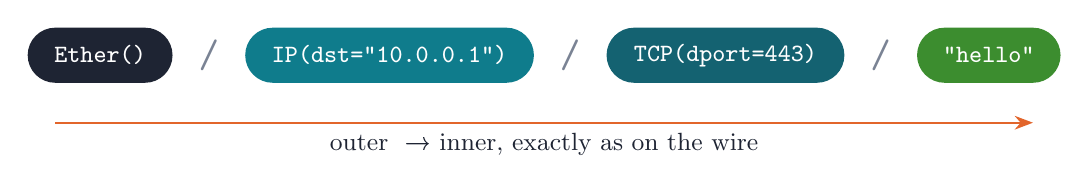
\begin{tikzpicture}[node distance=2mm]
  \node[layer=ink] (e) {Ether()};
  \node[slash, right=of e] (s1) {/};
  \node[layer=wire, right=of s1] (i) {IP(dst="10.0.0.1")};
  \node[slash, right=of i] (s2) {/};
  \node[layer=wire!70!ink, right=of s2] (t) {TCP(dport=443)};
  \node[slash, right=of t] (s3) {/};
  \node[layer=leaf, right=of s3] (p) {"hello"};
  \draw[-{Stealth}, spark, thick] ([yshift=-5mm]e.south west) --
     node[below, font=\small, text=ink] {outer \ \textrightarrow\ inner, exactly as on the wire}
     ([yshift=-5mm]p.south east);
\end{tikzpicture}

\bigskip
\raggedright
Each layer tells the one before it who comes next:
\begin{itemize}
  \item \texttt{Ether.type} becomes 0x0800 because IP follows,
  \item \texttt{IP.proto} becomes 6 because TCP follows,
  \item \texttt{IP.len} and both checksums cover everything after them.
\end{itemize}
A bare string at the end is a raw payload.
\end{frame}

% ────────────────────────────────────────────────────────────────────────────
\begin{frame}[fragile]{Look inside: \cmd{hexdump}, \cmd{raw}, \cmd{ls}}
\begin{term}
@@pcapsh >>>@@ hexdump(IP(dst="10.0.0.1")/ICMP()/"hi!")
0000  45 00 00 1F 00 01 00 00  40 01 F1 DB 7F 00 00 01  E.......@.......
0010  0A 00 00 01 08 00 6E 96  00 00 00 00 68 69 21     ......n.....hi!

@@pcapsh >>>@@ raw(IP()/UDP())
'E\x00\x00\x1c\x00\x01\x00\x00@\x11|\xce\x7f\x00\x00\x01\x7f\x00\x00\x01\x005\x005...'

@@pcapsh >>>@@ ls(ARP)
ARP fields:
  htype   uint16   1                    [ETHERNET=0x1]
  op      uint16   1                    [REQUEST=0x1, REPLY=0x2]
  sha     mac      00:00:00:00:00:00
  spa     ip4      0.0.0.0              ~~...~~
\end{term}
\tip{\cmd{ls()} with no argument lists every protocol pcapsh knows.}
\end{frame}

% ────────────────────────────────────────────────────────────────────────────
\begin{frame}[fragile]{Speaking the values}
\begin{columns}[T]
\column{0.5\textwidth}
\textbf{Numbers \& maths}
\begin{lstlisting}
TCP(dport=0x1BB)
UDP(sport=49000+7)
IP(id=0x100*2+1)
\end{lstlisting}
\textbf{Addresses are strings}
\begin{lstlisting}
IP(src="192.0.2.1")
Ether(src="02:00:c0:00:02:01")
\end{lstlisting}
\column{0.5\textwidth}
\textbf{Escapes in strings}
\begin{lstlisting}
"GET / HTTP/1.0\r\n\r\n"
"\xfeSMB binary \x00 ok"
\end{lstlisting}
\textbf{Flags \& names}
\begin{lstlisting}
TCP(flags="SA")      # SYN+ACK
TCP(flags=0x12)      # same thing
ARP(op=REPLY)        # enum name
DNSQR(qtype=MX)
\end{lstlisting}
\end{columns}
\tip{\texttt{/} is reserved for stacking, so maths has \texttt{+ - *} but no division.}
\end{frame}

% ────────────────────────────────────────────────────────────────────────────
\begin{frame}[fragile]{Variables: name it, reuse it, stack it}
\begin{lstlisting}
c = Ether(src="02:00:0a:00:01:01")/IP(src="10.0.1.1",dst="10.0.0.1")
v = Ether(src="02:00:0a:00:00:01")/IP(src="10.0.0.1",dst="10.0.1.1")

wrpcap("chat.pcapng", c/UDP(dport=9999)/"ping")
wrpcap("chat.pcapng", v/UDP(sport=9999)/"pong")
\end{lstlisting}
\begin{itemize}
  \item A variable holds a packet, raw bytes, a TCP session or a number.
  \item \alert{A stored packet is a layer}: \texttt{c/UDP(...)} keeps building on it.
  \item Define the two endpoints once and every later line stays short.
\end{itemize}
\end{frame}

% ────────────────────────────────────────────────────────────────────────────
\begin{frame}[fragile]{Long packet? Keep typing}
A statement carries on while a bracket is open or a line ends with \texttt{/} or \texttt{,}:
\begin{lstlisting}
answer = IP(src="8.8.8.8", dst="192.168.1.10")/
         UDP(sport=53, dport=54321)/
         DNS(id=0xC0DE, qr=1, rd=1, ra=1,
             qd=DNSQR(qname="pcapsh.rocks"),            # the question
             an=DNSRR(rrname="pcapsh.rocks", type=A,    # the answer
                      ttl=300, rdata="10.13.37.1"),
             ancount=1)
\end{lstlisting}
\begin{itemize}
  \item Comments on each line are fine; brackets inside strings do not count.
  \item In the REPL the prompt turns into \texttt{...}; an empty line submits.
  \item Wireshark hex dumps can be pasted over several lines into \cmd{fromhex("...")}.
\end{itemize}
\end{frame}

% ────────────────────────────────────────────────────────────────────────────
\begin{frame}[fragile]{From shell to Wireshark}
\begin{lstlisting}
wrpcap("hello.pcapng", Ether()/IP(dst="10.0.0.1")/ICMP()/"hi!")
wrpcap("hello.pcapng", Ether()/IP(src="10.0.0.1")/ICMP(type=0)/"hi!")
\end{lstlisting}
\begin{itemize}
  \item First call creates the file, \alert{later calls append}.
  \item Always Ethernet link type: an \texttt{Ether()} is added if you skipped it.
\end{itemize}
\begin{term}
$ wireshark hello.pcapng          ~~# or: tshark -r hello.pcapng~~
\end{term}
\tip{Appending is handy but sticky: \texttt{rm} the file before a fresh run.}
\end{frame}

% ════════════════════════════════════════════════════════════════════════════
\section{Protocols, the fun ones}

\begin{frame}[fragile]{DNS without tears}
\begin{lstlisting}
q  = IP(src="192.168.1.10",dst="8.8.8.8")/UDP(sport=54321,dport=53)
r  = IP(src="8.8.8.8",dst="192.168.1.10")/UDP(sport=53,dport=54321)
ask = DNSQR(qname="pcapsh.rocks")
ans = DNSRR(rrname="pcapsh.rocks",type=A,ttl=300,rdata="10.13.37.1")

wrpcap("dns.pcapng", q/DNS(id=0xC0DE,rd=1,qd=ask))
wrpcap("dns.pcapng", r/DNS(id=0xC0DE,qr=1,rd=1,ra=1,qd=ask,an=ans,ancount=1))
\end{lstlisting}
\begin{term}
$ tshark -r dns.pcapng
 1  192.168.1.10 → 8.8.8.8  DNS  Standard query 0xc0de A pcapsh.rocks
 2  8.8.8.8 → 192.168.1.10  DNS  Standard query response 0xc0de ... @@A 10.13.37.1@@
\end{term}
\tip{Passing \texttt{qd=} bumps \texttt{qdcount} for you; answers need \texttt{ancount=1}.}
\end{frame}

% ────────────────────────────────────────────────────────────────────────────
\begin{frame}[fragile]{Who has 10.0.0.1? Tell 10.0.0.100}
\begin{lstlisting}
wrpcap("arp.pcapng", Ether()/ARP(op=REQUEST, spa="10.0.0.100", tpa="10.0.0.1"))
wrpcap("arp.pcapng", Ether()/ARP(op=REPLY, sha="aa:bb:cc:dd:ee:01",
                                 spa="10.0.0.1", tpa="10.0.0.100"))
\end{lstlisting}
\tip{\texttt{Ether.type} follows the next layer: 0x0806 here, 0x0800 before IP.}

\medskip
\textbf{TCP options are fields too:}
\begin{lstlisting}
IP(dst="10.0.0.1")/TCP(dport=443,flags="S",mss=1460,sack_perm=1)
\end{lstlisting}
\begin{term}
40000 → 443 [SYN] Seq=0 Win=8192 Len=0 @@MSS=1460 SACK_PERM@@
\end{term}
\end{frame}

% ────────────────────────────────────────────────────────────────────────────
\begin{frame}[fragile]{Packet inception: tunnels}
\begin{lstlisting}
# a TCP SYN, in Ethernet, in VXLAN, in UDP, in IP
wrpcap("vxlan.pcapng", IP(src="10.0.0.1",dst="10.0.0.2")/
    UDP(sport=49152,dport=4789)/VXLAN()/
    Ether(src="02:aa:00:00:00:01")/IP(src="172.16.0.1",dst="172.16.0.2")/
    TCP(sport=40000,dport=8080,flags="S"))

# GRE: IPv4 carried over IPv4
wrpcap("gre.pcapng", IP(src="10.0.0.1",dst="10.0.0.2")/GRE(proto=IPV4)/
    IP(src="192.168.1.1",dst="192.168.2.1")/TCP(dport=80,flags="S"))
\end{lstlisting}
\centering
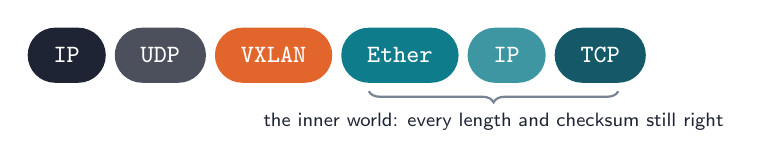
\begin{tikzpicture}[node distance=1mm, every node/.style={font=\ttfamily\scriptsize}]
  \node[layer=ink] (a) {IP};
  \node[layer=ink!80, right=of a] (b) {UDP};
  \node[layer=spark, right=of b] (c) {VXLAN};
  \node[layer=wire, right=of c] (d) {Ether};
  \node[layer=wire!80, right=of d] (e) {IP};
  \node[layer=wire!60!ink, right=of e] (f) {TCP};
  \draw[decorate, decoration={brace, amplitude=4pt, mirror}, thick, dim]
     ([yshift=-1mm]d.south west) -- node[below=4pt, text=ink, font=\scriptsize\sffamily]
     {the inner world: every length and checksum still right} ([yshift=-1mm]f.south east);
\end{tikzpicture}
\end{frame}

% ────────────────────────────────────────────────────────────────────────────
\begin{frame}[fragile]{Break it on purpose}
Lengths and checksums are computed \emph{unless you set them}. Fuzzers, IDS tests
and dissector bugs love this:
\begin{lstlisting}
wrpcap("evil.pcapng", IP(dst="10.0.0.1",ttl=0,chksum=0xdead)/
                      UDP(dport=53,len=4)/"oops")
\end{lstlisting}
\begin{term}
$ tshark -r evil.pcapng -o ip.check_checksum:TRUE -V
    [Expert Info (Note/Sequence): "Time To Live" only 0]
    [Expert Info (Error/Checksum): @@Bad checksum [should be 0x31cb]@@]
 1  127.0.0.1 → 10.0.0.1  UDP  53 → 53 @@[BAD UDP LENGTH 4 < 8]@@
\end{term}
\tip{Same trick for \texttt{IP(len=...)}, \texttt{IP(proto=...)}, \texttt{TCP(chksum=...)}, \texttt{Ether(type=...)}.}
\end{frame}

% ────────────────────────────────────────────────────────────────────────────
\begin{frame}[fragile]{75+ protocols ship in the box}
Native C layers plus \texttt{.posa} definitions loaded at start-up; try \cmd{ls()} and \cmd{ls(NAME)}.

\medskip
\footnotesize
\begin{columns}[T]
\column{0.24\textwidth}
\textbf{\textcolor{wire}{LAN}}\\ ARP, STP, CDP, LACP, 802.1Q, EAPOL, VRRP, HSRP, PPPoE
\column{0.24\textwidth}
\textbf{\textcolor{wire}{Internet}}\\ DNS, DHCP, NTP, IPv6, GRE, VXLAN, MPLS, BGP, OSPF, SCTP
\column{0.24\textwidth}
\textbf{\textcolor{wire}{Enterprise}}\\ SMB2, DCERPC, LDAP, Kerberos, RADIUS, NBNS, RDP, IKEv2
\column{0.24\textwidth}
\textbf{\textcolor{wire}{IoT \& industry}}\\ ModbusTCP, DNP3, BACnet, MQTT, CoAP, OpenFlow, PTPv2, Wake-on-LAN
\end{columns}
\normalsize
\bigskip
\begin{lstlisting}
IP()/TCP(dport=445)/NBT()/SMB2(command=READ, tree_id=1)
IP()/UDP(sport=49152,dport=1812)/RADIUS(code=ACCESS_REQUEST, identifier=7)
\end{lstlisting}
\end{frame}

% ════════════════════════════════════════════════════════════════════════════
\section{Scripts: write once, capture forever}

\begin{frame}[fragile]{A script is just the lines you typed}
\begin{lstlisting}
#!/usr/bin/env pcapsh
# ping.pcapsh -- two echo request/reply pairs
a = IP(src="10.0.0.1",dst="10.0.0.2")
b = IP(src="10.0.0.2",dst="10.0.0.1")
wrpcap("ping.pcapng", a/ICMP(type=8,id=1,seq=1)/"hello")
wrpcap("ping.pcapng", b/ICMP(type=0,id=1,seq=1)/"hello")
wrpcap("ping.pcapng", a/ICMP(type=8,id=1,seq=2)/"hello")
wrpcap("ping.pcapng", b/ICMP(type=0,id=1,seq=2)/"hello")
\end{lstlisting}
\begin{term}
$ chmod +x ping.pcapsh && ./ping.pcapsh
$ pcapsh -o lab42.pcapng ping.pcapsh   ~~# same script, different output file~~
$ pcapsh -e 'hexdump(IP()/ICMP())'      ~~# one-liner from any shell~~
\end{term}
\end{frame}

% ────────────────────────────────────────────────────────────────────────────
\begin{frame}[fragile]{Loops: a port scan in two lines}
\begin{lstlisting}
t = IP(src="10.0.0.66",dst="10.0.0.1")
for $p in range(20, 26):
    wrpcap("sweep.pcapng", t/TCP(sport=40000+$p,dport=$p,flags="S"))
\end{lstlisting}
\begin{columns}[T]
\column{0.42\textwidth}
\small
\begin{tabular}{@{}ll@{}}
\toprule
\texttt{range(n)} & 1 \ldots\ n \\
\texttt{range(a,b)} & a \ldots\ b-1 \\
\texttt{range(a,b,s)} & a, a+s, \ldots \\
\bottomrule
\end{tabular}

\smallskip
Indented lines form the body.
\column{0.55\textwidth}
\begin{term}
$ pcapsh sweep.pcapsh
$ tshark -r sweep.pcapng
10.0.0.66 → 10.0.0.1  40020 → 20 [SYN]
10.0.0.66 → 10.0.0.1  40021 → 21 [SYN]
10.0.0.66 → 10.0.0.1  40022 → 22 [SYN]
~~...~~
10.0.0.66 → 10.0.0.1  40025 → 25 [SYN]
\end{term}
\end{columns}
\tip{\texttt{range(n)} counts from \alert{1}, like packet numbers. \texttt{\$p} works in numeric fields only.}
\end{frame}

% ────────────────────────────────────────────────────────────────────────────
\begin{frame}[fragile]{Generate traffic by the bucket}
\begin{lstlisting}
# 20 NTP clients hitting one server, from ephemeral ports
cli = IP(src="10.0.1.1",dst="10.0.0.2")
srv = IP(src="10.0.0.2",dst="10.0.1.1")
for $i in range(20):
    wrpcap("ntp.pcapng", cli/UDP(sport=49151+$i,dport=123)/
                         NTP(li_vn_mode=CLIENT))
    wrpcap("ntp.pcapng", srv/UDP(sport=123,dport=49151+$i)/
                         NTP(li_vn_mode=SERVER,stratum=1))

# 50 DNS queries, each with its own ports and ids
q = DNSQR(qname="example.org")
for $i in range(50):
    wrpcap("dns50.pcapng", IP(dst="9.9.9.9",id=$i)/UDP(sport=50000+$i)/
                           DNS(id=$i*7,rd=1,qd=q))
\end{lstlisting}
\tip{Offset your ports (\texttt{49151+\$i}): \texttt{sport=\$i} lands on Echo, Discard, Chargen\ldots}
\end{frame}

% ════════════════════════════════════════════════════════════════════════════
\section{TCP that talks back}

\begin{frame}[fragile]{Hand-made TCP is a maths exam}
\begin{lstlisting}
TCP(flags="S",  seq=1000)
TCP(flags="SA", seq=5000, ack=1001)
TCP(flags="A",  seq=1001, ack=5001)
TCP(flags="PA", seq=1001, ack=5001)/"GET / HTTP/1.1\r\n\r\n"
TCP(flags="PA", seq=5001, ack=1019)/"HTTP/1.1 200 OK..."   # 1019? 1020? hmm
\end{lstlisting}
\pause
\begin{center}
\Large Let the shell do the counting. \faSmileWink[regular]
\end{center}
\end{frame}

% ────────────────────────────────────────────────────────────────────────────
\begin{frame}[fragile]{\cmd{TCPSession}: a whole web visit}
\begin{columns}[T]
\column{0.50\textwidth}
\begin{lstlisting}[basicstyle=\ttfamily\scriptsize\color{ink}]
s = TCPSession("192.168.1.100", "93.184.216.34",
               54321, 80)
wrpcap("http.pcapng", syn(s))
wrpcap("http.pcapng", syn_ack(s))
wrpcap("http.pcapng", ack(s))
wrpcap("http.pcapng", client_send(s,
    "GET / HTTP/1.1\r\nHost: example.com\r\n\r\n"))
wrpcap("http.pcapng", server_send(s,
    "HTTP/1.1 200 OK\r\nContent-Length: 3\r\n\r\nhi!"))
wrpcap("http.pcapng", client_fin(s))
wrpcap("http.pcapng", server_fin_ack(s))
\end{lstlisting}
\column{0.48\textwidth}
\begin{term}[basicstyle=\ttfamily\scriptsize\color{termfg}]
$ tshark -r http.pcapng
1 TCP   54321 → 80 [SYN] Seq=0
2 TCP   80 → 54321 [SYN, ACK] Seq=0 Ack=1
3 TCP   54321 → 80 [ACK] Seq=1 Ack=1
4 HTTP  @@GET / HTTP/1.1@@
5 HTTP  @@HTTP/1.1 200 OK@@
6 TCP   54321 → 80 [FIN, ACK] Seq=38 Ack=42
7 TCP   80 → 54321 [FIN, ACK] Seq=42 Ack=39
\end{term}
\small Every seq and ack lines up, so Wireshark's \emph{Follow TCP Stream}
replays the whole conversation.
\end{columns}
\end{frame}

% ────────────────────────────────────────────────────────────────────────────
\begin{frame}[fragile]{The session cheat sheet}
\centering
\begin{tabular}{@{}lll@{}}
\toprule
\textbf{Function} & \textbf{Direction} & \textbf{Flags} \\
\midrule
\cmd{syn(s)}                    & client \textrightarrow\ server & S \\
\cmd{syn\_ack(s)}               & server \textrightarrow\ client & SA \\
\cmd{ack(s)} / \cmd{tcp\_ack(s)} & client \textrightarrow\ server & A \\
\cmd{client\_send(s, data)}     & client \textrightarrow\ server & PA \\
\cmd{server\_send(s, data)}     & server \textrightarrow\ client & PA \\
\cmd{client\_fin(s)}            & client \textrightarrow\ server & FA \\
\cmd{server\_fin\_ack(s)}       & server \textrightarrow\ client & FA \\
\bottomrule
\end{tabular}

\bigskip
\raggedright
\begin{itemize}
  \item Each call returns a full Ether/IP/TCP packet and advances seq/ack.
  \item MACs derive from IPs, so endpoints are stable across a capture.
  \item Run several sessions at once; they interleave in write order.
  \item \texttt{data} may be bytes too: \texttt{client\_send(s, raw(SMB2()))}.
\end{itemize}
\end{frame}

% ────────────────────────────────────────────────────────────────────────────
\begin{frame}[fragile]{TLS, minus the secrets}
Handshake records ready to drop after TCP; NULL cipher, so Wireshark sees everything.
\begin{lstlisting}
c = IP(src="10.0.1.1",dst="10.0.0.1")
v = IP(src="10.0.0.1",dst="10.0.1.1")
wrpcap("tls.pcapng", c/TCP(sport=50000,dport=636,flags="PA",seq=1,ack=1)/
                     TLS_CLIENT_HELLO())
wrpcap("tls.pcapng", v/TCP(sport=636,dport=50000,flags="PA",seq=1,ack=51)/
                     TLS_SERVER_HELLO())
wrpcap("tls.pcapng", c/TCP(sport=50000,dport=636,flags="PA",seq=51,ack=48)/
                     TLS()/LDAP(op_tag=BIND_REQUEST))
\end{lstlisting}
\begin{term}
 1  10.0.1.1 → 10.0.0.1  TLSv1.2  Client Hello
 2  10.0.0.1 → 10.0.1.1  TLSv1.2  Server Hello
 3  10.0.1.1 → 10.0.0.1  TLSv1.2  Application Data
\end{term}
\tip{\texttt{TLS()} wraps whatever follows. Record sizes: Hello 50/47, Certificate 12, CCS 6, Finished 21.}
\end{frame}

% ════════════════════════════════════════════════════════════════════════════
\section{Reading, dissecting, editing}

\begin{frame}[fragile]{\cmd{rdpcap}: tshark-lite with display filters}
\begin{term}
@@pcapsh >>>@@ rdpcap("sweep.pcapng", "tcp.dstport in {22..24}")
  3  ~~…~~  TCP  10.0.0.66 → 10.0.0.1  40022 → 22 [SYN] Seq=3735928320 ~~…~~
  4  ~~…~~  TCP  10.0.0.66 → 10.0.0.1  40023 → 23 [SYN] Seq=3735928320 ~~…~~
  5  ~~…~~  TCP  10.0.0.66 → 10.0.0.1  40024 → 24 [SYN] Seq=3735928320 ~~…~~
3 / 6 packet(s) matched
\end{term}
\small
\begin{columns}[T]
\column{0.5\textwidth}
\begin{lstlisting}
"dns"
"ip.addr == 192.168.0.0/16"
"tcp.port in {80, 443}"
"dns && !(ip.src == 8.8.8.8)"
\end{lstlisting}
\column{0.5\textwidth}
\begin{lstlisting}
"udp.dstport >= 1024 && udp"
"eth.src[0:3] == 02:00:c0"
"http.request"
"tcp.flags.syn == 1"
\end{lstlisting}
\end{columns}
\tip{Reads pcap and pcapng. \texttt{-k keylog} (or \texttt{\$SSLKEYLOGFILE}) loads TLS keys.}
\end{frame}

% ────────────────────────────────────────────────────────────────────────────
\begin{frame}[fragile]{Paste hex, get meaning: \cmd{fromhex} + \cmd{show}}
Copy bytes from Wireshark (\emph{Copy \textrightarrow\ as Hex Dump}), paste, name the stack:
\begin{term}
@@pcapsh >>>@@ d = fromhex("45 00 00 34 00 01 00 00 40 11 f6 c4 c0 a8 01 05
                    08 08 08 08 c3 a8 00 35 00 20 41 a1 12 34 01 00
                    00 01 00 00 00 00 00 00")
@@pcapsh >>>@@ show("IP/UDP/DNS", d)
<IP src=192.168.1.5 dst=8.8.8.8 ttl=64 proto=17(UDP) len=52 |
<UDP sport=50088 dport=53 len=32 |
<DNS id=4660 flags=0x0100 qdcount=1 ancount=0 nscount=0 arcount=0 |
\end{term}
\begin{itemize}
  \item \cmd{fromhex} eats plain streams, spaced bytes, or full Wireshark dumps
        with offsets and ASCII.
  \item \cmd{show} walks the stack; IP and TCP options are skipped by their length fields.
\end{itemize}
\end{frame}

% ────────────────────────────────────────────────────────────────────────────
\begin{frame}[fragile]{Packet surgery on an existing capture}
\begin{lstlisting}
# dissect the first three packets
for $n in range(3):
    show("Ether/IP/TCP", frompcapng("sweep.pcapng", $n))

# swap packet 3 for a RST, in place
replacepkt("sweep.pcapng", 3,
           IP(src="10.0.0.66",dst="10.0.0.1")/TCP(sport=40022,dport=22,flags="R"))
\end{lstlisting}
\begin{term}
Replaced packet #3 in sweep.pcapng (54 bytes)
@@pcapsh >>>@@ rdpcap("sweep.pcapng")
  2  ~~…~~  TCP  10.0.0.66 → 10.0.0.1  40021 → 21 [SYN] Seq=3735928320 ~~…~~
  3  ~~…~~  TCP  10.0.0.66 → 10.0.0.1  40022 → 22 @@[RST]@@ Seq=0 ~~…~~
  4  ~~…~~  TCP  10.0.0.66 → 10.0.0.1  40023 → 23 [SYN] Seq=3735928320 ~~…~~
\end{term}
\tip{\cmd{frompcapng(file, n)} returns raw bytes: feed them to \cmd{show}, \cmd{hexdump} or \cmd{wrpcap}.}
\end{frame}

% ════════════════════════════════════════════════════════════════════════════
\section{Invent your own protocol}

\begin{frame}[fragile]{The Pizza Ordering Protocol\texttrademark}
\begin{columns}[T]
\column{0.38\textwidth}
\begin{lstlisting}[basicstyle=\ttfamily\scriptsize\color{ink}]
protocol Pizza
    uint8 size defaults(2)
        SMALL  = 1
        MEDIUM = 2
        LARGE  = 3
    uint8 topping defaults(1)
        CHEESE    = 1
        PEPPERONI = 2
        PINEAPPLE = 3
    uint16 quantity defaults(1)
    cstring note defaults("extra hot")
end
\end{lstlisting}
\column{0.60\textwidth}
\begin{lstlisting}[basicstyle=\ttfamily\footnotesize\color{ink}]
p = IP(dst="10.0.0.42")/UDP(sport=50000,dport=8080)/
    Pizza(size=LARGE, topping=PINEAPPLE,
          quantity=2)
hexdump(p)
\end{lstlisting}
\begin{term}[basicstyle=\ttfamily\scriptsize\color{termfg}]
0010  0A 00 00 2A C3 50 1F 90  00 16 79 36 @@03 03 00 02@@
0020  @@65 78 74 72 61 20 68 6F  74 00@@         @@extra hot.@@
\end{term}
\small Usable the moment \texttt{end} is read: build it, dump it, \cmd{ls(Pizza)} it,
and dissect it:
\end{columns}
\begin{term}
@@pcapsh >>>@@ show("Pizza", fromhex("03 03 00 02 6e 6f 20 61 6e 63 68 6f 76 69 65 73 00"))
<Pizza size=LARGE(3) topping=PINEAPPLE(3) quantity=2 note='no anchovies' |
\end{term}
\end{frame}

% ────────────────────────────────────────────────────────────────────────────
\begin{frame}[fragile]{Keep it in a \texttt{.posa} file}
\begin{columns}[T]
\column{0.36\textwidth}
\begin{lstlisting}[basicstyle=\ttfamily\scriptsize\color{ink}]
# game.posa
Object<GAME> GAME_HELLO
    uint8 opcode defaults(1)
        HELLO = 1
    cstring player defaults("neo")

Object<GAME> GAME_SCORE
    uint8 opcode defaults(2)
        SCORE = 2
    uint32 points defaults(0)
\end{lstlisting}
\column{0.62\textwidth}
\small
\texttt{Object<GAME>} groups messages: \cmd{show("GAME", ...)} picks the
member whose opcode matches.
\begin{term}[basicstyle=\ttfamily\scriptsize\color{termfg}]
$ pcapsh game.posa
@@>>>@@ show("GAME", fromhex("02 00 00 05 39"))
<GAME_SCORE opcode=SCORE(2) points=1337 |
@@>>>@@ show("GAME", fromhex("01 74 72 69 6e 69 74 79 00"))
<GAME_HELLO opcode=HELLO(1) player='trinity' |
@@>>>@@ hexdump(GAME_HELLO(player="morpheus"))
0000  01 6D 6F 72 70 68 65 75  73 00     .morpheus.
\end{term}
\end{columns}
\tip{Load with \texttt{-p}, \cmd{load("game.posa")}, or forever via \texttt{\textasciitilde/.pcapsh\_protos.posa}.}
\end{frame}

% ────────────────────────────────────────────────────────────────────────────
\begin{frame}{The posa toolbox}
\centering
\begin{tabular}{@{}ll@{}}
\toprule
\textbf{Type} & \textbf{What it is} \\
\midrule
\texttt{uint8 uint16 uint32 uint64} & big-endian integers \\
\texttt{le\_uint16 le\_uint32 le\_uint64} & little-endian (hello, SMB2) \\
\texttt{mac}, \texttt{ip4} & addresses: \texttt{defaults(10.0.0.1)} \\
\texttt{bytes<N>}, \texttt{str<N>} & fixed width, zero padded \\
\texttt{cstring} & NUL-terminated text \\
\texttt{string x until "\textbackslash r\textbackslash n"} & text up to a delimiter (HTTP, SIP\ldots) \\
\texttt{enum<uint8>} & integer with names \\
\bottomrule
\end{tabular}

\bigskip
Indented \texttt{NAME = value} lines under a field give it enum names. \\
Full language reference: \texttt{doc/posa.md}.
\end{frame}

% ════════════════════════════════════════════════════════════════════════════
\section{Wrapping up}

\begin{frame}[fragile]{Coming from Scapy? You already know this}
\centering
\small
\begin{tabular}{@{}lll@{}}
\toprule
\textbf{Task} & \textbf{Scapy} & \textbf{pcapsh} \\
\midrule
Build      & \texttt{IP()/TCP()}           & \texttt{IP()/TCP()} \\
Inspect    & \texttt{hexdump(p)}, \texttt{ls(TCP)} & \texttt{hexdump(p)}, \texttt{ls(TCP)} \\
Save       & \texttt{wrpcap("f", p)}       & \texttt{wrpcap("f", p)} \textit{(appends)} \\
Read       & \texttt{rdpcap("f")}          & \texttt{rdpcap("f", "filter")} \\
Loop       & \texttt{for i in range(10):}  & \texttt{for \$i in range(10):} \textit{(1..10)} \\
New proto  & a Python class                & 5 lines of \texttt{protocol\ldots end} \\
TCP state  & do it yourself                & \texttt{TCPSession} \\
Multi-line & Python rules                  & open bracket or trailing \texttt{/} \\
Start-up   & Python + imports              & one C binary \\
\bottomrule
\end{tabular}

\bigskip
\raggedright
pcapsh builds and writes files; it does not send packets on the wire.
\end{frame}

% ────────────────────────────────────────────────────────────────────────────
\begin{frame}{Your turn: five challenges}
\begin{enumerate}
  \item[\faDice] \textbf{Ping pong.} Ten ICMP echo request/reply pairs with
        \texttt{seq=1..10}, in one loop.
  \item[\faGlobe] \textbf{DNS liar.} A query for \texttt{bank.example} and an
        answer pointing it to \texttt{10.66.6.6}.
  \item[\faDoorOpen] \textbf{Knock knock.} SYNs to ports 7000, 8000, 9000, then a
        full \texttt{TCPSession} to port 22.
  \item[\faMailBulk] \textbf{Syslog storm.} 100 RFC 3164 messages:
        \texttt{UDP(dport=514)/"<38>Oct 24 10:00:01 host app: hi"}.
  \item[\faPizzaSlice] \textbf{Pizza over TCP.} Order three pizzas through
        \texttt{client\_send(s, raw(Pizza(\ldots)))} and read them back with
        \cmd{show}.
\end{enumerate}
\bigskip
\centering
Check every answer with \texttt{tshark -r} or \cmd{rdpcap}.
\end{frame}

% ────────────────────────────────────────────────────────────────────────────
\begin{frame}[fragile]{Pocket reference}
\small
\begin{columns}[T]
\column{0.5\textwidth}
\textbf{Run}
\begin{term}
pcapsh                    ~~REPL~~
pcapsh file.pcapsh        ~~script~~
pcapsh -e 'EXPR'          ~~one-shot~~
pcapsh -p x.posa          ~~extra protocols~~
pcapsh -o out.pcapng s.pcapsh
pcapsh --version
\end{term}
\textbf{Build}\quad \texttt{A()/B(f=v)/"payload"}
\column{0.5\textwidth}
\textbf{Functions}
\begin{term}
hexdump(p)  raw(p)  ls([P])
wrpcap(file, p)
rdpcap(file [, filter])
frompcapng(file, n)
replacepkt(file, n, p)
fromhex("..")  show("A/B", bytes)
load("x.posa")  RandShort()
\end{term}
\end{columns}
\bigskip
\centering
\Large\texttt{man pcapsh} \quad \normalsize and \texttt{help()} inside the shell
\end{frame}

% ────────────────────────────────────────────────────────────────────────────
{
\setbeamercolor{background canvas}{bg=ink}
\begin{frame}[standout]
  \Huge Now go make\\[2mm] some packets.\\[6mm]
  \Large \texttt{\$ pcapsh}
\end{frame}
}

\end{document}
